%guassian with conficence region and with y axis 
\begin{center}
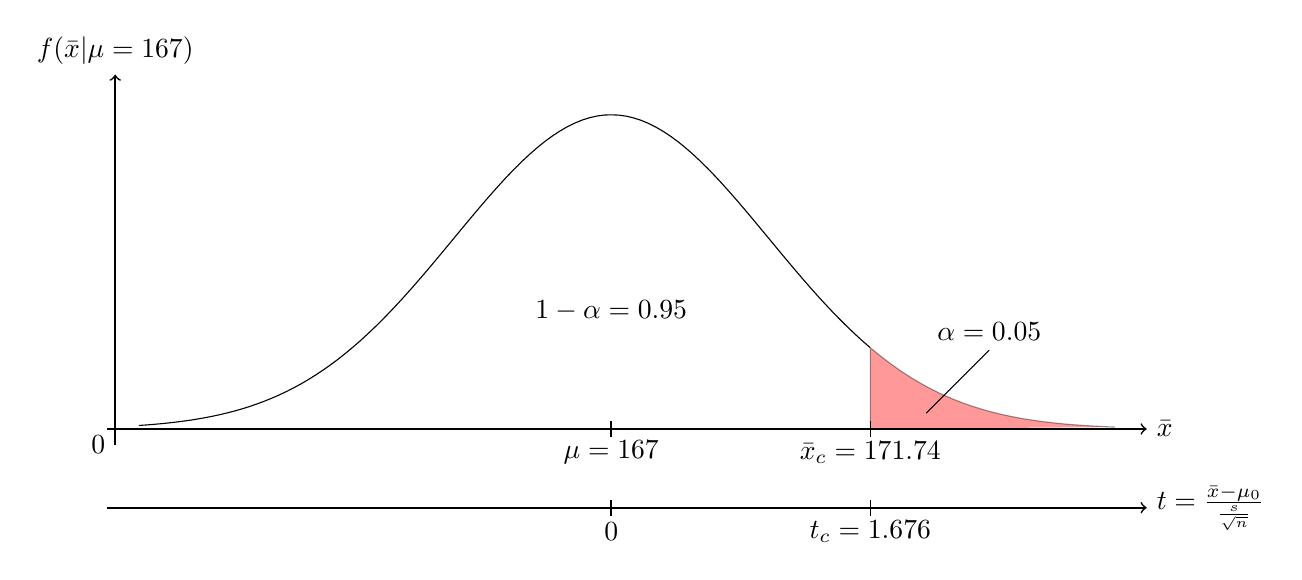
\begin{tikzpicture}[scale=2, y=5cm]
\draw[domain=-3:1.645] plot[id=gauss1, samples=100] (\x,{1/sqrt(2*pi)*exp(-0.5*(\x)^2)});   
\draw[domain=1.645:3.2,fill=red,opacity=0.4] (1.645,0) --
plot[id=gauss3, samples=25] (\x,{1/sqrt(2*pi)*exp(-0.5*(\x)^2)});
\draw (1.645,-0.01) -- (1.645,0.01);    % tick
\node at (1.645,-0.03) {$\bar{x}_c = 171.74$};
\draw[->, semithick] (-3.2,0) -- (3.4,0) node[right]
{$\bar{x}$}; % x-axis 1  
\draw[->, semithick] (-3.2,-0.1) -- (3.4,-0.1) node[right] {$t=\frac{\bar{x}-\mu_0}{\frac{s}{\sqrt{n}}}$}; % x-axis 2

%y-axis
\draw[->, semithick] (-3.15,-0.02) node[left] {$0$} -- (-3.15,0.45)
node[above] {$f(\bar{x}|\mu=167)$}; % y-axis

\draw[-,semithick] (0,-0.01) -- (0,0.01); % zero tick on x
\draw[-,semithick] (0,-0.11) -- (0,0.-0.09); % zero tick on z
\node at (0,-0.03) {$\mu = 167$};
\node at (0,-0.13) {$0$};
\draw[-,semithick] (1.645,-0.11) -- (1.645,-0.09);
\node at (1.645,-0.13)  {$t_c = 1.676$};
% annotate alphas
\node at (0,0.15) {$1 - \alpha = 0.95$};
\draw (2,0.02) -- (2.4,0.1) node[above] {$\alpha = 0.05$};
\end{tikzpicture} 
\end{center}